\documentclass[12pt]{article}

\usepackage[margin=2cm]{geometry}
\usepackage{amsmath}
\usepackage{multicol}
\usepackage{nopageno}
\usepackage{SIunits}
\usepackage{graphicx}
\usepackage{enumerate}
\usepackage{enumitem}
%\usepackage{mathabx}
\usepackage{wasysym}


% for making bond drawings
\usepackage{chemfig}
% Global bond settings
\setchemfig{
  atom sep=18pt,               % fixed bond length
  double bond sep=2pt,       % spacing between the two bars
  bond style={line width=0.8pt}
}


% for centering figures on page while in an enumerated/itemized list:
\usepackage{changepage} % in the preamble
\makeatletter
\newenvironment{centerinpage}
  {%
    \par\noindent
    \hspace*{-\@totalleftmargin}% back to page margin (covers all nested list indents)
    \begin{minipage}{\textwidth}% fixed to page width (ignores widened \linewidth)
      \centering
  }
  {%
    \end{minipage}\par
  }
\makeatother

%%%%%%%%%%%%%%%%%%%%%%%%%%%%%%%%%%%%%%%%%%%%%%%%%%%%%
% For putting links in the document (both to sections and hyperlinks)
\usepackage{hyperref}
\usepackage{url}
\hypersetup{
    colorlinks=true,     % false: boxed links; true: colored links
    linkcolor=red,       % color of internal links
    citecolor=blue,      % color of links to bibliography
    filecolor=blue,      % color of file links
    urlcolor=blue        % color of external links
}
% below, use \url{http://www.nytimes.com} (they will be urlcolor)
%%%%%%%%%%%%%%%%%%%%%%%%%%%%%%%%%%%%%%%%%%%%%%%%%%%%%


%%%%%%%%%%%%%%%%%%%%%%%%%%%%%%%%%%%%%%%%%%%%%%%%%%%%%
% for the events page boxes

% boxed regions
\usepackage{tcolorbox}
\tcbuselibrary{skins,breakable}

% fonts & spacing
\usepackage{lmodern}
\usepackage{microtype}
\usepackage{calc}


% small helper macros (adjust these)
\newcommand{\boxheight}{4.2cm}   % height for each event box
\newcommand{\boxfont}{\scriptsize} % change to \tiny or \footnotesize as desired
\newcommand{\linelen}{0.95\linewidth} % timeline line length

%%%%%%%%%%%%%%%%%%%%%%%%%%%%%%%%%%%%%%%%%%%%%%%%%%%%%
\newcommand{\rmd}{\ensuremath{{\rm d}}}
%\newcommand{\vv}[1]{\ensuremath{\vec{#1}}}
\newcommand{\vv}[1]{\ensuremath{\mathbf{#1}}}
\newcommand{\ee}[1]{\ensuremath{\mathbf{e}_{#1}}}
%%%%%%%%%%%%%%%%%%%%%%%%%%%%%%%%%%%%%%%%%%%%%%%%%%%%%



\begin{document}

\begin{center}
{\Large Evaporation, dew point, fog, frost}
\end{center}
%%%%%%%%%%%%%%%%%%%%%%%%%%%%%%%%%%%%%%%%%%%%%%%%
%%%%%%%%%%%%%      overview         %%%%%%%%%%%%%%%%%%%%%
%%%%%%%%%%%%%%%%%%%%%%%%%%%%%%%%%%%%%%%%%%%%%%%%

\noindent In lab this week we examine the {\bf psychrometric chart} --- relating relative humidity to absolute humidity --- and the {\bf phase diagram} for water --- depicting the coexistence curve between liquid water and water vapor near 0$\degree$C. Both are reproduced in this packet on a later page, along with the larger phase diagram for water that we saw in Lab 07.  \\[-6pt]

\noindent The smaller phase diagram is useful for understanding the evaporation of water exposed to air, because in that case the relevant pressure is not the atmospheric pressure, $p_\text{atm}$, but instead the {\bf partial pressure}, $e$, defined as
	%
	\begin{equation*}
	e = f  \times p_\text{atm} = \left( \frac{n_{\text{H}_2 \text{O}}}{n_{\text{H}_2 \text{O}} + n_\text{dry air}} \right) \times p_\text{atm}\,,
	\end{equation*}
	%
where you can see that partial pressure is found by multiplying the atmospheric pressure by $f$, the {\bf mole fraction of water in air}.  In lab you re-write this mole fraction in terms of the {\bf absolute humidity}, AH.  That new expression is:
	%
	\begin{equation*}
	\begin{split}
	e &= \left( \frac{ 
	\frac{m_{\text{H}_2 \text{O}}}{m_\text{dry air}}  \cdot  \frac{M_\text{dry air}}{M_{\text{H}_2 \text{O}}} 
	}
	{ \frac{m_{\text{H}_2 \text{O}}}{m_\text{dry air}}  \cdot \frac{M_\text{dry air}}{M_{\text{H}_2 \text{O}}}  + 1 } \right) \times p_\text{atm} \\
	& \\
	& =  
	\left(
	\frac{ \text{AH} \cdot 1.6}{ \text{AH} \cdot 1.6 + 1} 
	\right) \times p_\text{atm}
	\end{split}
	\end{equation*}
	%
where the mass ratio  $\frac{m_{\text{H}_2 \text{O}}}{m_\text{dry air}}$  is the absolute humidity read from the vertical axis of the psychrometric chart (but expressed as a pure ratio, e.g., $\unit{7}{\gram} / \unit{1}{\kilo\gram} = \unit{7}{\gram} / \unit{1000}{\gram} = 0.007$), and where the ratio of the molar masses is $M_\text{dry air} / M_{\text{H}_2 \text{O}}  =  28.8/18 = 1.6$.  So now you can:
	%
	\begin{itemize}
	\item Look up or measure the ``weather conditions'': relative humidity (\%) and ambient temperature.
	\item Use the psychrometric chart to convert these to an absolute humidity value, AH.
	\item Calculate the associated partial pressure of water in air, using the final equation above.
	\item Determine the vaporization temperature (liquid to vapor) from the phase diagram.
	\end{itemize}
	%
This vaporization temperature --- which is called ``the boiling point'' in a {\em pure} water liquid-vapor transition --- is called the {\bf dew point} when considering water exposed to air.


\newpage
%%%%%%%%%%%%%%%%%%%%%%%%%%%%%%%%%%%%%%%%%%%%%%%%
%%%%%%%%%%%%%      questions         %%%%%%%%%%%%%%%%%%%%%
%%%%%%%%%%%%%%%%%%%%%%%%%%%%%%%%%%%%%%%%%%%%%%%%

\begin{enumerate}

\item {\bf The dew point and water evaporation} Let's calculate the dew point temperature for a few different locations with diverse weather conditions.  In each case, draw a horizontal line on the phase diagram provided corresponding to your calculated partial pressure (label the line its location/conditions). Draw a dot on the line where it crosses the coexistence curve and a star on the line at the associated ambient temperature value.
	%
	\begin{enumerate}
	\item Let's start with ``indoor conditions.'' Modern heating and air conditioning is designed not only to keep the temperature at ``room temperature'' (look this up in $\degree$C), but also a comfortable 50\% relative humidity.  
	\item Now let's do Allendale/Grand Rapids yesterday in the afternoon. You can google for ``\verb|NWS 7 day grand rapids|'' and then navigate to the ``3 day History'' link (remember to convert temperatures from Fahrenheit to Celsius\ldots google can do this for you). Do you remember, was it comfortable outside (both in terms of temperature and humidity)?  
	\item On the search box of the NWS page, navigate to a different city where you expect that conditions were less humid than here.  Again look up their afternoon data. Alternatively, you might look for a very dry day in a very dry city\footnote{For example, you could google for ``when is it hottest and driest in Phoenix'' and then use a historical weather database like \url{https://www.wunderground.com/history} to obtain their afternoon temperature and humidity, under ``Daily Observations.''}.
	\item Repeat the previous, but for a location with very humid conditions.
	\item Use the website in the footnote for (c) to find the conditions in Grand Rapids on a typical winter afternoon (e.g., in January).  In these conditions (when temperature is below 0$\degree$C) you can still find an absolute humidity from the psychrometric chart, but will need to look at the larger phase diagram.  You will find that there is no longer a transition from liquid to vapor, nor a dew point, but there is a ``frost point.'' Find that value and discuss its meaning.
	\end{enumerate}

\item {\bf Why dew?}  Using our understanding of evaporation developed in the previous question and in lab, let's try to answer some qualitative questions about our surroundings.  Feel free to look for advice from your instructor or the web, but try to give answers that reference the technical understanding we have from the phase diagram.
	%
	\begin{enumerate}
	\item In lab this week we do an experiment where the temperature of a beaker of water is slowly lowered by the introduction of ice.  What did you observe (or would you expect to observe) on the outside of the beaker and when? 
	\item Look up the temperature of a standard refrigerator.  If you remove a jar of olives from the fridge, do you expect to see condensation?  Where does the ``condensation'' come from?
	\item Look up the temperature of a standard freezer.  If you remove a tub of ice cream from the freezer, do you expect to see condensation?  What do you expect to see and why?
	\item Why is there dew on your car on some mornings and not on others?  Think about this question in terms of the dew point you worked with in question 1 and in terms of condensation.  Is the temperature of the air the same as the temperature of the car?  How can this occur?  Where does the dew come from?
	\item If I have dew on my car windshield I usually find that using the wipers clears it up only for a moment.  Why is that the case, and what controls should you use to clear it up completely?
	\item When does frost appear on your car?  
	\item What does it mean when you ``see your breath''?  Remember that water vapor is invisible, and clouds are formed when the vapor condenses into tiny liquid droplets (or ice particles).
	\item On a cool fall morning, I saw mist rising off a pond on my drive in to work.  Why is this happening?
	\item What is fog and what are the conditions for it to occur?
	\item Examining your responses to Question (1), what does relative humidity seem to indicate?  Why is this measure important to us in terms of how we feel on a given day?  Why is a high relative humidity uncomfortable?
	\end{enumerate}


%\item {\bf Radiative-Convective Equilibrium Temperature} In prior weeks we made estimates of the Earth's equilibrium temperature.  In fact this is the driving question of the first half of the course: What do we expect to be the temperature of the Earth?  Let's review our prior results and then push forward to a new (and basically final) answer using the mechanism of energy transfer by evaporation.
%	%
%	\begin{enumerate}
%	\item st
%	\end{enumerate}

\end{enumerate}

\newpage

%%%%%%%%%%%%%%%%%%%%%%%%%%%%%%
\mbox{}
\newpage
%%%%%%%%%%%%%%%%%%%%%%%%%%%%%%

%%%%%%%%%%%%%%%%%%%%%%%%%%%%%%%%%%%%%%%%%%%%%%%%%%%%
%%%%%%%%%%               phase diagram and psychrometric chart              %%%%%%%%%%%%%
%%%%%%%%%%%%%%%%%%%%%%%%%%%%%%%%%%%%%%%%%%%%%%%%%%%%


\begin{figure}
\centering
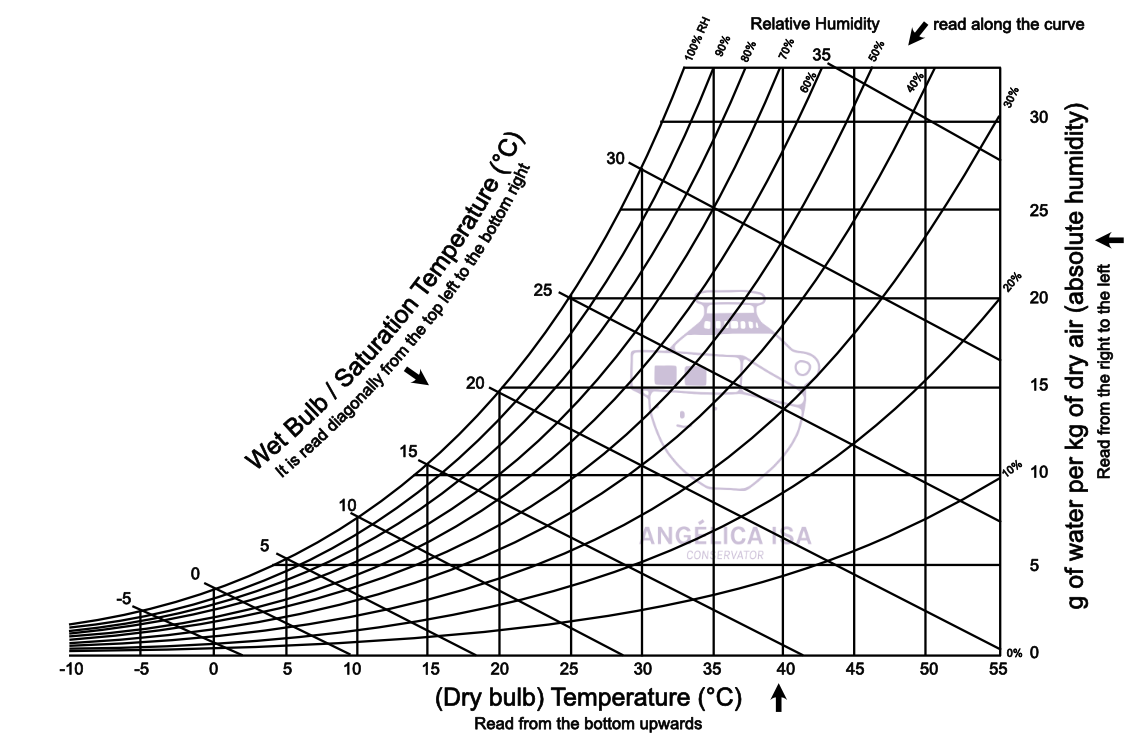
\includegraphics[width=0.95 \textwidth]{images/08_psychrometric_angelica-isa.png}\\
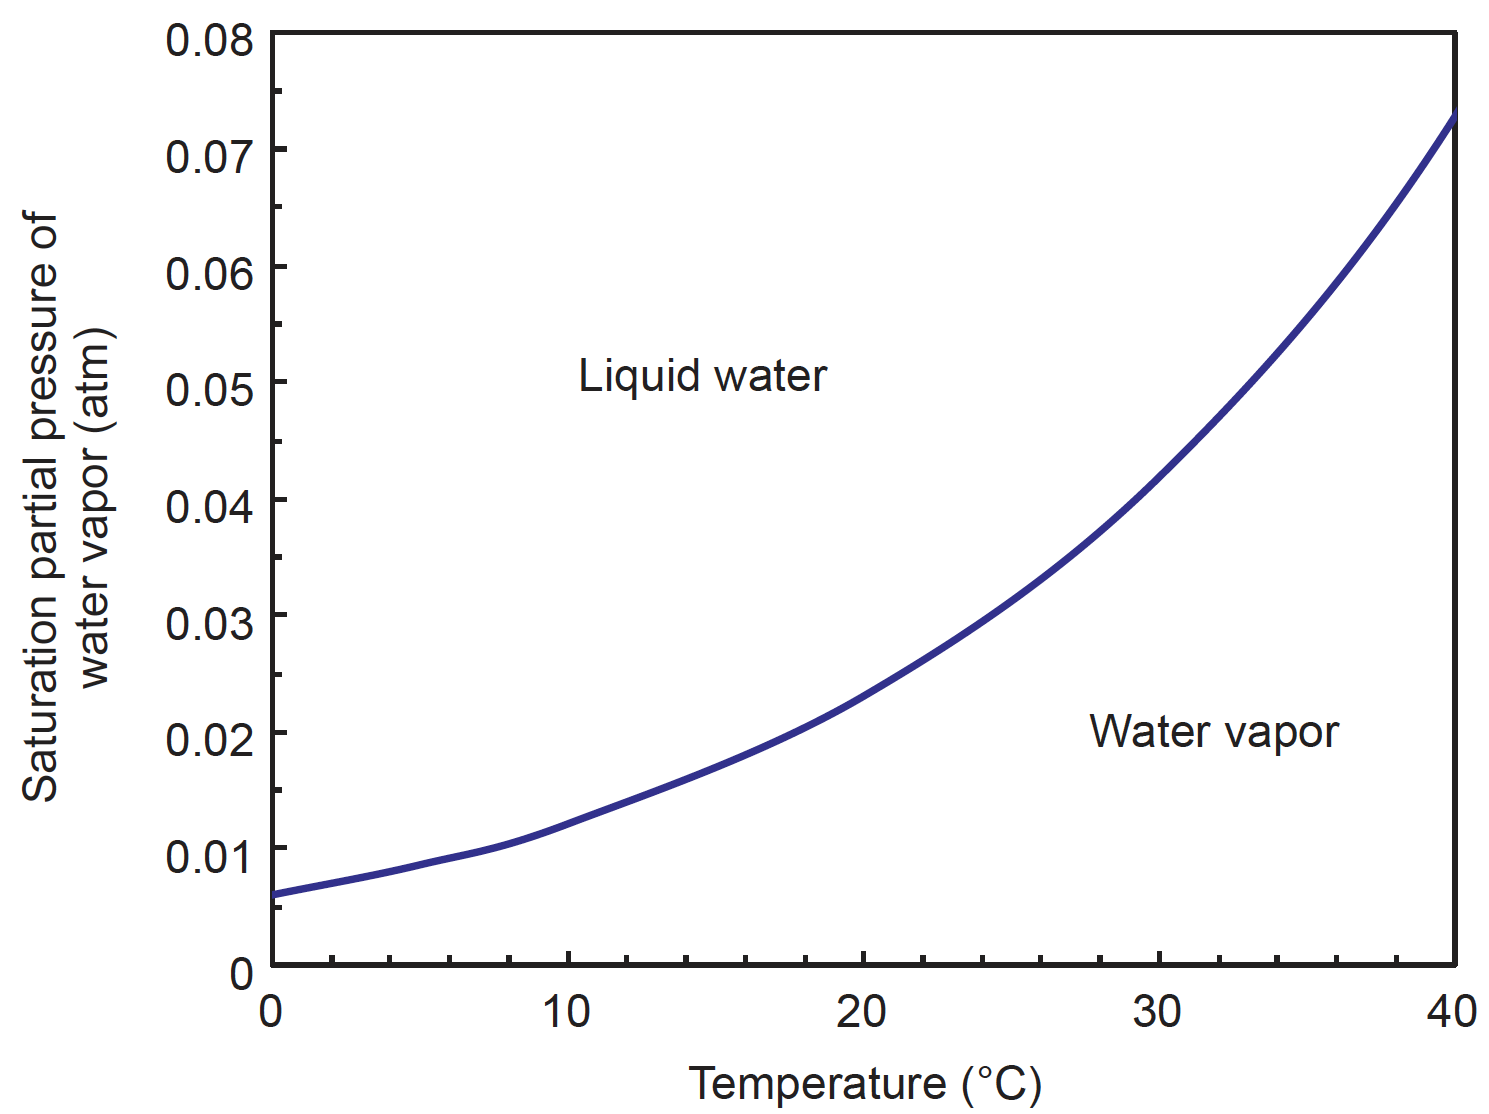
\includegraphics[width=0.95 \textwidth]{images/08_pressure-vs-temperature-clausius-clapeyron_mathez-fig-1-2_no-caption.png}
\caption{ \label{fig:08_psychrometric-and-phase-diagrams}
{\bf Top}: Psychrometric chart for water at standard pressure conditions $\unit{1}{atm} = \unit{101}{\kilo\pascal}$ (from angelicaisa.com). {\bf Bottom}: Phase transition coexistence curve for water near the triple point (from Mathez \& Smerdon).
}
\end{figure}



\newpage
%%%%%%%%%%%%%%%%%%%%%%%%%%%%%%%%%%%%%%%%%%%%%%%%%%%%
%%%%%%%%%%                   larger phase diagram for water                        %%%%%%%%%%%%%
%%%%%%%%%%%%%%%%%%%%%%%%%%%%%%%%%%%%%%%%%%%%%%%%%%%%


\begin{figure}[h]
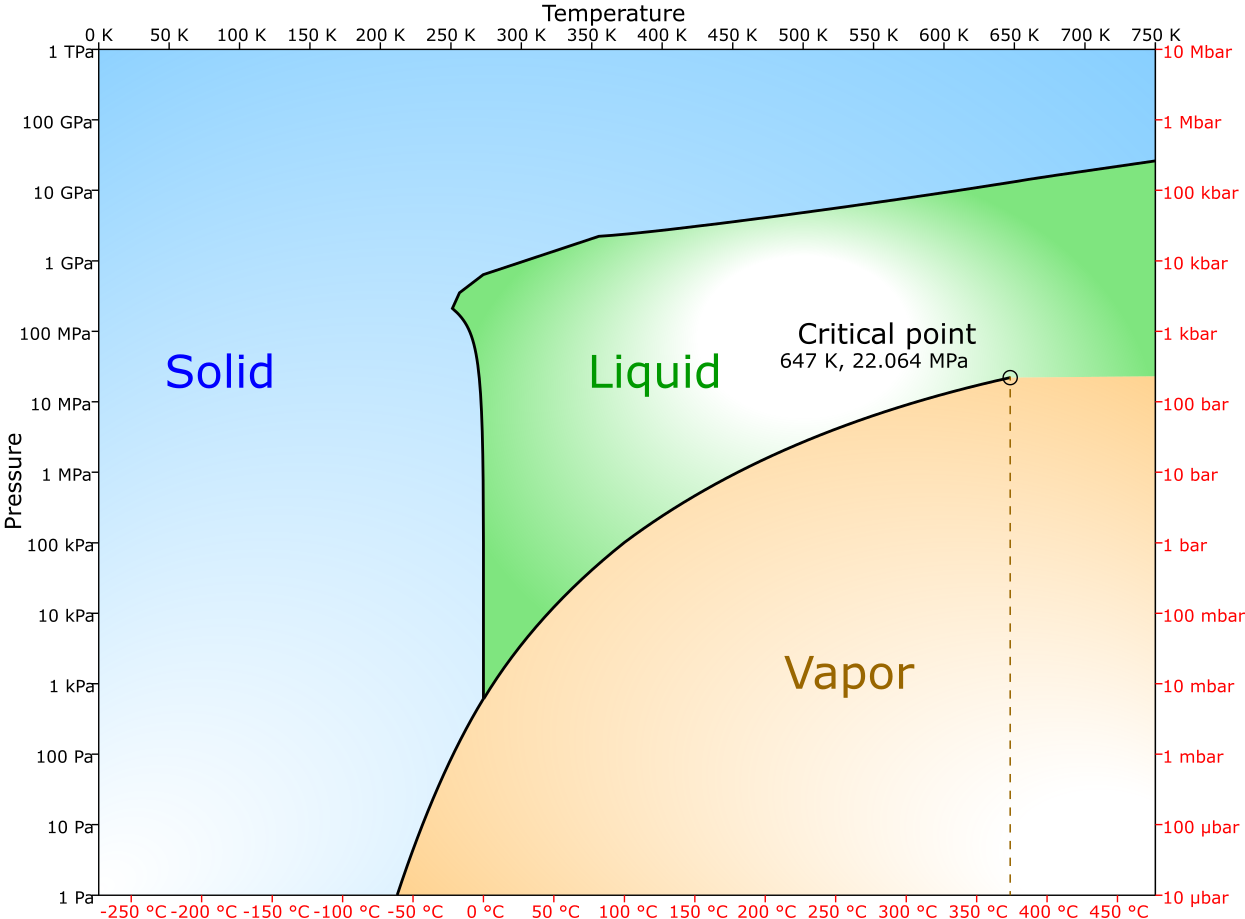
\includegraphics[width=\textheight, angle=90]{images/07_phase-diagram-of-water-simplified_wikimedia-Cmglee_edited.png}
\caption{\label{fig:07_phase-diagram-water}
Phase diagram of water. (Adapted from wikimedia upload by Hokanomono and Cmglee)
}
\end{figure}


%%%%%%%%%%%%%%%%%%%%%%%%%%%%%%%%%%%%%%%%%%%%%%%%%%%%
%%%%%%%%%%                                  References                                %%%%%%%%%%%%%%%%
%%%%%%%%%%%%%%%%%%%%%%%%%%%%%%%%%%%%%%%%%%%%%%%%%%%%
%\noindent {\bf Data Sources}: 



\end{document}
